\documentclass[a4paper]{usiinfbachelorproject}

\captionsetup{labelfont={bf}}
\usepackage{float}
\usepackage{amsmath}
\usepackage{graphicx}
\usepackage{enumitem}
\usepackage{booktabs}
\usepackage{hyperref}

\author{POLAD BAKHISHZADE}

\title{\textbf{LLM as Code-Correctness Judge}}
\subtitle{Unveiling the Causes of Large-Language-Model Failures when Assessing Java Code}
\versiondate{\today}

\begin{committee}
  \advisor[Università della Svizzera italiana, Switzerland]{ }{Gabriele}{Bavota}
  \coadvisor[Università della Svizzera italiana, Switzerland]{ }{Giuseppe}{Crupi}
\end{committee}

% ——————————————————————————— ABSTRACT
\abstract{
\textbf{Context.}  
Large Language Models (LLMs) are increasingly being used in software development tasks such as code generation, explanation, and bug fixing. An emerging frontier is the use of LLMs for code review—specifically, assessing whether a given implementation is functionally correct. This requires reasoning over both the specification and the code, making it a strong benchmark for code understanding.\\
\\[2pt]
\textbf{Objective.}  
This study investigates how the quality and quantity of natural-language context affect the ability of LLMs to assess code correctness. We ask: \emph{What kind of descriptive information helps or harms the model’s ability to judge whether a function is correct?}\\
\\[2pt]
\textbf{Method.}  
We extend the Java subset of the \textsc{CoderEval} benchmark by systematically enriching it with five structured documentation layers—ranging from brief summaries to formal pre/post-conditions. Each of 362 functions is paired with one correct and one incorrect candidate implementation. We then prompt three open LLMs—Qwen-0.5B, Qwen-1.5B, and DeepSeek-1.3B—to act as zero-shot code judges, under multiple prompt configurations.\\
\\[2pt]
\textbf{Findings.}  
The results reveal that different models respond differently to added context: smaller models benefit from concise behavioral descriptions but often degrade when presented with verbose examples or formal constraints. In contrast, larger models leverage detailed descriptions to reduce mistakes and achieve more reliable judgments. Some layers, such as examples, can introduce confusion and accuracy drop depending on the model.\\
\\[2pt]
\textbf{Outcome.}  
The study highlights the importance of model-specific prompt design and shows that more documentation is not always better. These insights can inform future systems that rely on LLMs for code quality assessment.\\
\\[2pt]
\textbf{Keywords}: LLMs; Code Review; Code Correctness; Prompt Engineering; Evaluation; Java; Dataset Enrichment
}

\begin{document}
\maketitle
\tableofcontents\newpage

% ——————————————————————————— 1 INTRODUCTION
\section{Introduction}\label{sec:intro}

\subsection{LLMs and the promise of autonomous code review}

Tools such as GitHub Copilot, ChatGPT Code Interpreter, and StarCoder have moved LLMs from research prototypes into the daily workflow of developers. Beyond generating or explaining code, a natural next milestone is \emph{autonomous code review}—having the model assess whether an implementation correctly matches a given specification. At the core of this task is the LLM’s ability to judge \textbf{functional correctness}.

\subsection{Why correctness judgement matters}

Failure to judge correctness accurately can cause critical issues in two major settings:

\begin{enumerate}[label=\textbf{S\arabic*},leftmargin=14pt,itemsep=0pt]
  \item \textbf{Pull-request triage}: Models that approve buggy code or reject valid patches mislead developers and reduce trust in automation.
  \item \textbf{Self-refinement loops}: Recent LLM-based code generators incorporate feedback loops where the model critiques and iteratively improves its own output. These loops are only effective if the internal judge is reliable.
\end{enumerate}

\subsection{Gaps in current understanding}

While LLMs have shown impressive results in generation and repair tasks, their reliability in correctness judgment remains underexplored. Moreover, existing benchmarks often include only short or vague natural-language descriptions, potentially limiting the model’s reasoning capability.

\subsection{Our hypothesis: prompt complexity vs. model capacity}

Intuitively, richer natural-language context should help LLMs reason more accurately. But overly verbose prompts may contain redundancy, ambiguity, or distractions. We hypothesize that:

\begin{quote}
\centering
\emph{Smaller models benefit from concise, focused descriptions, while larger models can exploit more detailed and structured context.}
\end{quote}

\subsection{Approach overview}

To test this hypothesis, we extended the \textsc{CoderEval} benchmark with five structured documentation layers:

\begin{itemize}[leftmargin=14pt]
  \item L1: one-line summary,
  \item L2: behavioral description,
  \item L3: signature semantics,
  \item L4: examples (input/output),
  \item L5: pre- and post-conditions.
\end{itemize}
We ran three instruction-tuned LLMs (Qwen-0.5B, Qwen-1.5B, DeepSeek-1.3B) on 362 function–candidate pairs, testing both \textit{cumulative} prompts (gradually adding more documentation layers) and \textit{ablation} prompts (removing one specific layer at a time to isolate its impact, if any). A unified evaluation pipeline was used to measure accuracy and confusion metrics.

\subsection{Key insights}

Our findings confirm the importance of tailoring prompts to model capacity:

\begin{itemize}[leftmargin=14pt]
  \item Small models improve with behavior descriptions but are easily misled by verbose context.
  \item Larger models leverage all five layers to reduce misclassifications and false negatives.
  \item Some documentation elements (e.g., examples) can hurt performance if not well-integrated.
\end{itemize}

\subsection*{Report structure}

Section~\ref{sec:related} reviews related literature.  
Section~\ref{sec:design} presents our study design and dataset enrichment pipeline.  
Section~\ref{sec:results} covers results from cumulative and ablation experiments.  
Section~\ref{sec:concl} concludes and outlines future directions.

% ——————————————————————————— 2 RELATED WORK
\section{Related Work}\label{sec:related}

The application of Large Language Models (LLMs) as evaluators in software engineering tasks has garnered significant attention. This section reviews pivotal studies that explore LLMs' capabilities in assessing code correctness, understanding, and alignment with coding preferences, providing context and contrast to our investigation into LLM-based code correctness judgment.

\subsection{LLMs as Judges: Datasets and Benchmarks}

\textbf{CodeUltraFeedback} by Weyssow et al.~\cite{weyssow2024codeultrafeedback} introduces a dataset comprising 10,000 coding instructions, each annotated with responses from 14 diverse LLMs. These responses are evaluated based on five coding preferences: instruction following, code explanation, code complexity and efficiency, code readability, and coding style. GPT-3.5 serves as the judge to rank these responses. The study demonstrates that fine-tuning models like CodeLlama-7B-Instruct using this dataset can outperform larger models in aligning with coding preferences and improving functional correctness on benchmarks like HumanEval+. This work underscores the potential of LLMs not only in code generation but also in nuanced evaluation tasks, aligning closely with our focus on LLMs as code correctness judges.\\
\\[2pt]
\textbf{CodeJudge-Eval} by Zhao et al.~\cite{zhao2024codejudgeeval} presents a benchmark designed to evaluate LLMs' code understanding abilities from the perspective of code judging rather than code generation. The benchmark includes tasks where models must determine the correctness of provided code solutions, including those with subtle errors or compilation issues. Evaluations of 12 prominent LLMs reveal that even state-of-the-art models struggle with this task, highlighting the need for improved code understanding in LLMs. This benchmark provides a direct comparison point for our study, emphasizing the challenges LLMs face in accurately assessing code correctness.\\
\\[2pt]
\textbf{ICE-Score} introduced by Zhuo~\cite{zhuo2023icescore} proposes an evaluation metric that instructs LLMs to assess code quality, addressing the limitations of traditional token-matching metrics like BLEU. ICE-Score correlates more strongly with functional correctness and human preferences, eliminating the need for test oracles or reference implementations. Evaluations across four programming languages demonstrate its effectiveness in aligning with human judgments. This approach aligns with our methodology of leveraging LLMs for code evaluation, reinforcing the viability of instruction-based assessment metrics.

\subsection{Understanding LLM Limitations in Code Evaluation}

\textbf{The Generative AI Paradox} by West et al.~\cite{west2023generative} explores the discrepancy between the generative capabilities of LLMs and their understanding of the generated content. The study finds that while models can produce outputs that surpass human performance, they often lack a deep understanding of the content, leading to brittleness and susceptibility to adversarial inputs. This paradox underscores the challenges in relying on LLMs for tasks that require genuine comprehension, a concern directly relevant to our investigation into LLM-based code correctness judgment.\\
\\[2pt]
\textbf{The Counterfeit Conundrum} by Gu et al.~\cite{gu2024counterfeit} investigates whether code language models can discern the nuances of their incorrect generations, termed "counterfeits." The study identifies three primary failure modes: models misclassify incorrect code as correct, struggle to reason about the execution behavior of counterfeits, and often fail to repair them effectively. These findings highlight the shallow understanding LLMs have of their erroneous outputs, emphasizing the need for improved evaluation mechanisms, as pursued in our research.

\subsection{LLMs in Educational Contexts and Evaluation Frameworks}

\textbf{Evaluating Language Models for Generating and Judging Programming Feedback} by Koutcheme et al.~\cite{koutcheme2025evaluating} assesses the efficiency of open-source LLMs in generating high-quality feedback for programming assignments and judging the quality of programming feedback. Their evaluations on a dataset of students' submissions to introductory Python programming exercises suggest that state-of-the-art open-source LLMs are nearly at the same level with proprietary models in both generating and assessing programming feedback. This finding underscores the potential of open-source models in educational contexts and the importance of further research in this area, complementing our focus on LLMs' evaluative capabilities.\\
\\[2pt]
\textbf{CodeJudge} by Tong and Zhang~\cite{tong2024codejudge} proposes a framework that leverages LLMs to evaluate the semantic correctness of generated code without relying on test cases. The approach involves guiding LLMs through a "slow thinking" process to perform in-depth evaluations. Experiments across four code generation datasets and five programming languages show that CodeJudge outperforms existing methods, achieving better results even with smaller models like Llama-3-8B-Instruct. This framework aligns with our objective of enhancing LLM-based code evaluation, offering insights into effective evaluation strategies.


% ——————————————————————————— 3 STUDY DESIGN
\section{Study Design}\label{sec:design}

\subsection*{Research question}
\noindent\textbf{RQ} -  
\emph{To what extent the information reported in the code description impact the ability of the LLMs to judge the correctness of a given code?}

\subsection{Models evaluated}\label{sec:models}
\begin{itemize}[leftmargin=12pt,itemsep=1pt]
  \item \textbf{Qwen-0.5B Instruct} (0.5 B params).  
  \item \textbf{Qwen-1.5B Instruct} (1.5 B).  
  \item \textbf{DeepSeek-Coder-1.3B Instruct}.  
\end{itemize}

\subsection{Dataset}\label{sec:dataset}
From the Java subset of \textsc{CoderEval}:
\begin{enumerate}[label=\alph*),leftmargin=14pt,itemsep=0pt]
  \item Removed noisy IDs.  
  \item For each remaining ID, selected one correct and one incorrect candidate (existing model outputs).  
\end{enumerate}
Final size: \textbf{362} rows (balanced).

\subsection{Documentation layers}\label{sec:layers}
\begin{description}[style=nextline,leftmargin=15pt]
  \item[L1] Summary (1 sentence).  
  \item[L2] Behaviour narrative (detailed summary).  
  \item[L3] Signature description (argument/return semantics).  
  \item[L4] Examples (I/O pairs).  
  \item[L5] Pre/post-conditions.  
\end{description}
ChatGPT-4o generated all layers for each of 181 Java functions.

\subsection{Prompt template}
\textbf{Constant preamble}: task, label scheme (`0/1`, no extra text).\\
\textbf{Variable payload}: selected layers + \textit{first line of candidate code} (argument/return).\\
\textbf{Generation}: temperature 0.2, max\_new\_tokens 20.

\subsection{Experimental conditions}
\textbf{Incremental} (5 runs):
\[
\text{L1};\; \text{L1+L2};\; \text{L1+L2+L3};\; \text{L1+L2+L3+L4};\; \text{L1+L2+L3+L4+L5}
\]
\textbf{Ablations}:
\[
\text{No L1};\; \text{No L2};\; \text{No L4};\; \text{No L5}
\]

\subsection{Metrics}
TP, TN, FP, FN; Accuracy = (TP+TN)/362.

\subsection{Project Repository}
\href{https://github.com/poladbachs/Bachelor-Thesis}{\texttt{github.com/poladbachs/Bachelor-Thesis}}.

% ——————————————————————————— 4 RESULTS
\section{Results \& Discussion}\label{sec:results}

%------------------------------------------------------------------
\subsection{Incremental enrichment (L1 $\rightarrow$ L5)}
%------------------------------------------------------------------

\begin{figure}[H]\centering
  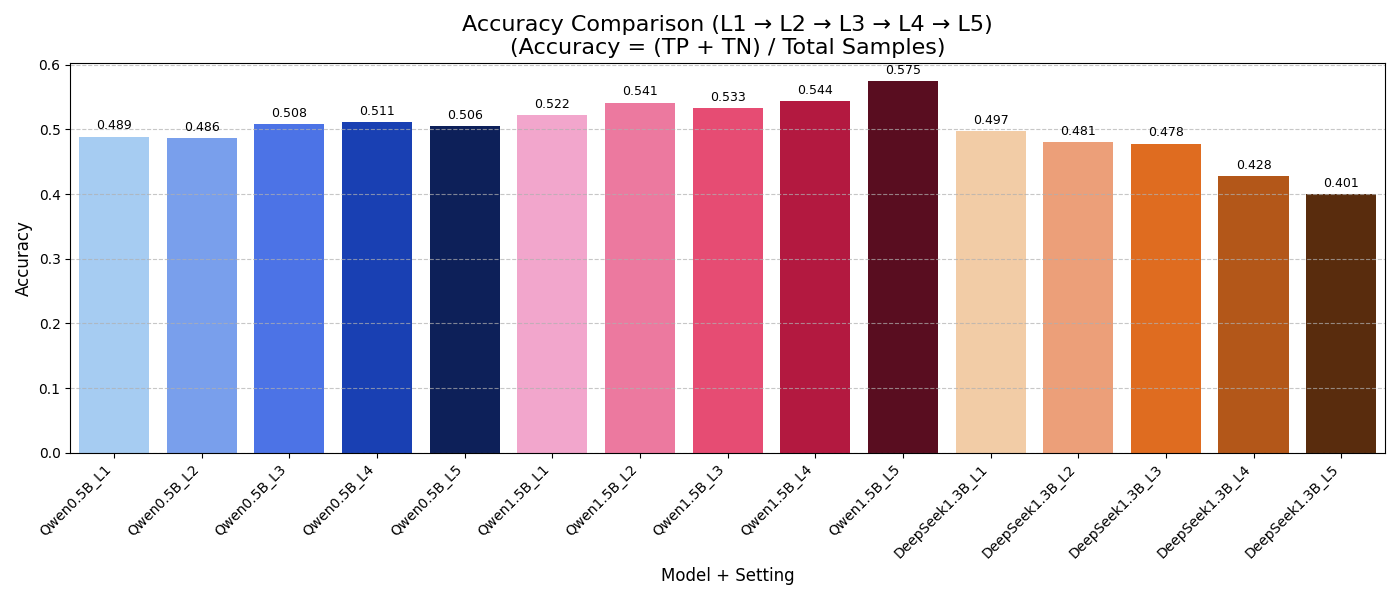
\includegraphics[width=0.95\linewidth]{figures/accuracy_comparison.png}
  \caption{Accuracy per model and documentation level.}
  \label{fig:acc-l1-l5}
\end{figure}

\paragraph*{Accuracy trends.}
We observe clear divergence in how each model responds to additional natural-language context:

\begin{itemize}[leftmargin=12pt]
  \item \textbf{Qwen-0.5B}: After stagnating on L1-L2, the model improves through L3 and L4, peaking at 0.511. L5 slightly degrades performance, suggesting diminishing returns or confusion from formal logic.
  
  \item \textbf{Qwen-1.5B}: Displays consistent benefit from each additional layer, rising steadily to 0.575 at L5. This model appears to handle verbosity well and leverages the full specification.

  \item \textbf{DeepSeek-1.3B}: Begins strong at 0.497 with minimal input, but drops with every added level—falling below 0.41 at L5. More context leads to worse performance, implying overload or poor instruction tuning for interpretive tasks.
\end{itemize}

These trends support our core hypothesis: smaller models benefit from concise cues, while larger models thrive on richer context. However, more detail is not universally helpful—its usefulness depends on model capacity and internal robustness to verbosity.

\vspace{0.8em}

% --------------------------- Qwen-0.5B
\begin{figure}[H]\centering
  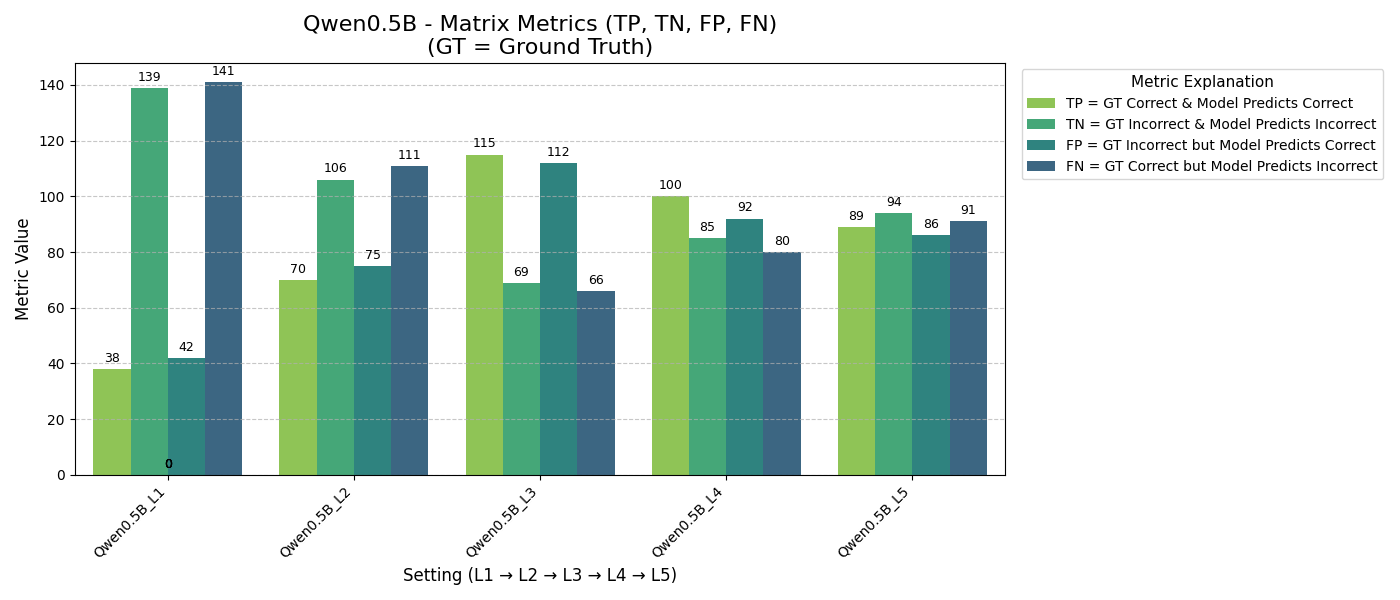
\includegraphics[width=\linewidth]{figures/Qwen0.5B_matrix_metrics.png}
  \caption{Confusion-matrix metrics — Qwen-0.5B.}
  \label{fig:q05-matrix}
\end{figure}

\paragraph*{Interpretation — Qwen-0.5B.}
Early stages (L1–L2) show a struggle to distinguish correct from incorrect implementations, with high false negatives. L3 and L4 reduce FN significantly, converting many correct cases into true positives. However, at L5 false positives creep back in, suggesting that formal conditions (pre/post) mislead the model or increase ambiguity. Overall, Qwen-0.5B needs concise clarity—too much structure destabilizes its judgment.

\vspace{0.8em}

% --------------------------- Qwen-1.5B
\begin{figure}[H]\centering
  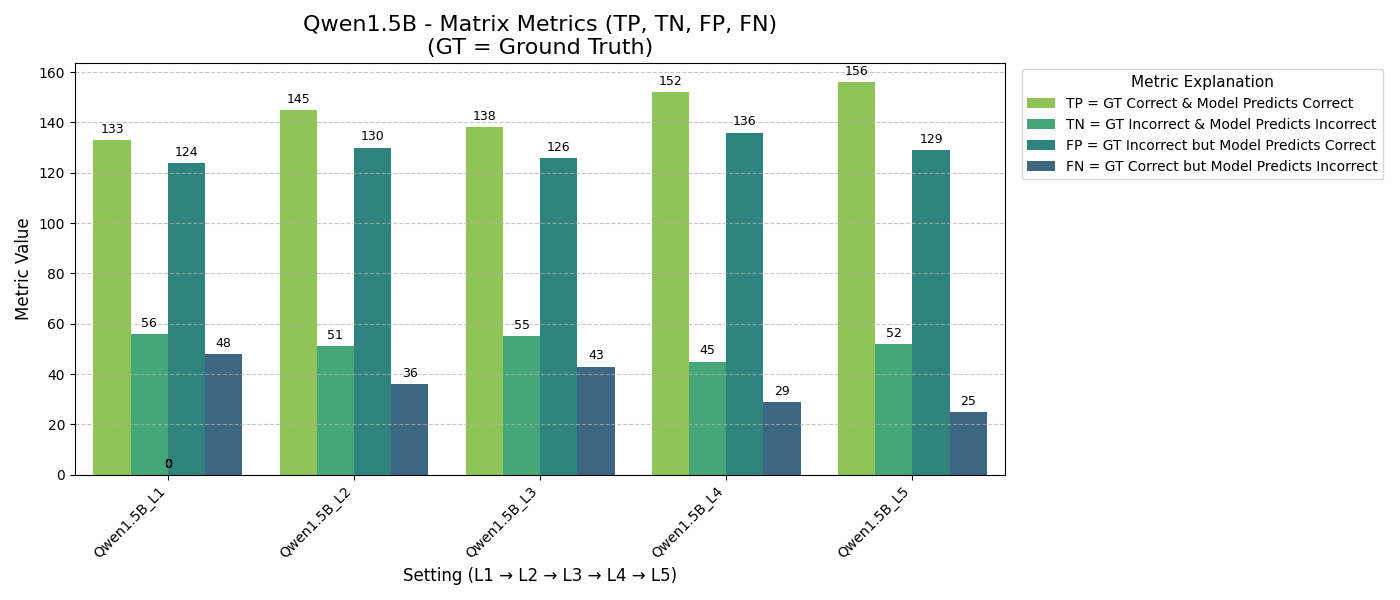
\includegraphics[width=\linewidth]{figures/Qwen1.5B_matrix_metrics.png}
  \caption{Confusion-matrix metrics — Qwen-1.5B.}
  \label{fig:q15-matrix}
\end{figure}

\paragraph*{Interpretation — Qwen-1.5B.}
The larger Qwen model handles incremental context with ease. As layers are added, false negatives drop sharply while true positives grow, especially after L4–L5. Pre/post-conditions help the model rule out wrong implementations without over-predicting correctness (FP stays stable). The balance between increased TP and maintained TN implies that Qwen-1.5B is the most context-aware model among the three.

\vspace{0.8em}

% --------------------------- DeepSeek-1.3B
\begin{figure}[H]\centering
  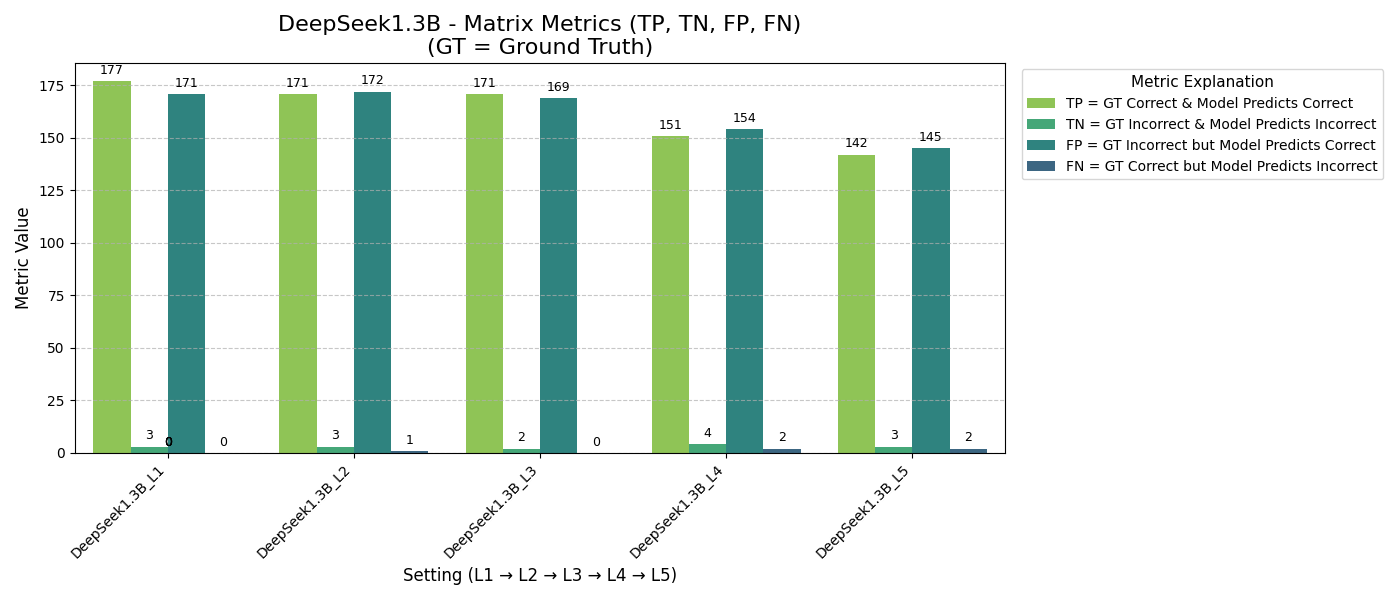
\includegraphics[width=\linewidth]{figures/DeepSeek1.3B_matrix_metrics.png}
  \caption{Confusion-matrix metrics — DeepSeek-1.3B.}
  \label{fig:ds-matrix}
\end{figure}

\paragraph*{Interpretation — DeepSeek-1.3B.}
Despite its comparable size, DeepSeek behaves like a brittle small model in judgment tasks. At L1 and L2, it achieves high TP with minimal FN. But starting at L3, false positives spike and true negatives collapse. This suggests that the added details—examples, constraints—shift attention away from core logic and confuse decision boundaries. It likely overfocuses on surface patterns in examples, falsely validating buggy code.



\subsection{Single-layer ablations}

\begin{table}[H]\centering
\caption{Accuracy after removing one layer. Values in parentheses show the change relative to the full prompt (L1--L5).}
\begin{tabular}{lccc}
\toprule
\textbf{Model} & \textbf{No L1} & \textbf{No L2} & \textbf{No L4} \\ \midrule
Qwen-0.5B  & 0.481 (-0.025) & \textbf{0.450 (-0.056)} & 0.494 (-0.012) \\
Qwen-1.5B  & 0.572 (-0.003) & 0.558 (-0.017) & 0.552 (-0.023) \\
DeepSeek-1.3B & \textbf{0.500 (+0.099)} & 0.434 (+0.034) & 0.428 (+0.028) \\
\bottomrule
\end{tabular}
\end{table}

\paragraph*{Interpretation.}
\begin{itemize}[leftmargin=12pt,itemsep=0pt]
  \item Removing behaviour (L2) cripples Qwen-0.5B (-5.6pp) $A \Rightarrow B$
 small model needs that layer.  
  \item Summary (L1) is useless or noisy for DeepSeek (+9.9pp when removed).  
  \item Qwen-1.5B tolerates all removals ($\leq$2pp), showing robustness.
\end{itemize}

\subsection{Compound ablations (illustrative)}

For space we discuss one illustrative combo per model:

\begin{itemize}[leftmargin=12pt]
  \item \textbf{Qwen-0.5B No L1 \& No L4}: accuracy 0.506 (-0.006 vs. full) — removing summary offsets example noise.  
  \item \textbf{Qwen-1.5B No L1 \& No L4}: 0.558 (-0.017) — examples help this model.  
  \item \textbf{DeepSeek No L2 \& No L4}: 0.478 (+0.078) — minimal prompt is best.  
\end{itemize}

\subsection{What makes a layer “noisy”?}
Manual error analysis highlights three patterns:

\begin{enumerate}[label=\alph*),leftmargin=15pt,itemsep=0pt]
  \item \textbf{Example bias}.  L4 lists only happy-path cases → model over-predicts “correct”.  
  \item \textbf{Narrative redundancy}.  L2 restates corner cases differently from L5, confusing alignment.  
  \item \textbf{Generic summaries}.  L1 adds little entropy; for DeepSeek it seems to trigger a “looks plausible → correct” bias.
\end{enumerate}

% ——————————————————————————— 5 CONCLUSIONS
\section{Conclusions \& Future Work}\label{sec:concl}

\begin{itemize}[leftmargin=12pt]
  \item Moderate enrichment (+behaviour, +signature) boosts small models (+8pp).  
  \item Verbose layers (examples, formal conditions) help mid-size models but harm 0.5 B and DeepSeek.  
  \item Removing noisy layers (summary or examples) can recover performance (DeepSeek +10pp).  
\end{itemize}

\textbf{Next steps}.  
\begin{enumerate}[label=\arabic*.]
  \item Fine-tune a 0.5 B checkpoint on the enriched dataset.  
  \item Auto-select minimal counter-examples to make L4 compact and balanced.  
  \item Extend to Python and larger open models (e.g.\ Llama-3-8B).  
\end{enumerate}

% ——————————————————————————— REFERENCES
\bibliographystyle{abbrv}
\bibliography{references}

\end{document}
